%% Fair UAM routing --- ICRA 2027 submission
%% Figures are pgfplots/TikZ in figs/*.tex, generated by ../harness/export_plot_data.py
%% from the CSVs in data/; tables in tables/ are generated by ../harness/analyze.py.
%% Neither is hand-edited.
\documentclass[conference]{IEEEtran}
\IEEEoverridecommandlockouts
% T1 so that XeTeX-based engines (Tectonic) set the body in Times as pdfLaTeX does;
% without it they fall back to Latin Modern and the page count is not comparable.
\usepackage[T1]{fontenc}

\usepackage{cite}
\usepackage{amsmath,amssymb,amsfonts}
% amsthm supplies the `proof' environment used for Proposition 1. IEEEtran does not
% define one (it has \IEEEproof), so this is required, not optional.
\usepackage{amsthm}
\usepackage{graphicx}
\usepackage{textcomp}
\usepackage{xcolor}
\usepackage{booktabs}
\usepackage{url}
\usepackage{pgfplots}
\usepackage{pgfplotstable}
\pgfplotsset{compat=1.18}
\usepgfplotslibrary{groupplots,fillbetween}
\usetikzlibrary{calc}
\usepackage[hidelinks]{hyperref}
% Generated by harness/export_plot_data.py from tex/data/*.csv. Do not edit.
\definecolor{fig-equal}{HTML}{0072B2}
\definecolor{fig-sufficientarian}{HTML}{E69F00}
\definecolor{fig-prioritarian}{HTML}{009E73}
\definecolor{fig-utilitarian}{HTML}{D55E00}
\definecolor{fig-proportional}{HTML}{CC79A7}
\definecolor{fig-baseline}{HTML}{555555}
\definecolor{fig-amb45}{HTML}{DCEEFB}
\definecolor{fig-amb55}{HTML}{F5F0D8}
\definecolor{fig-amb65}{HTML}{F2D6C4}
\definecolor{fig-route}{HTML}{B3261E}
\definecolor{fig-prot}{HTML}{1C6B52}
\definecolor{fig-t45}{HTML}{1F77B4}
\definecolor{fig-t55}{HTML}{FF7F0E}
\definecolor{fig-t65}{HTML}{2CA02C}
\pgfplotsset{
  paperaxis/.style={scale only axis, axis lines*=left,
    font=\footnotesize, tick label style={font=\footnotesize},
    label style={font=\scriptsize}, tick align=outside,
    tick style={black!70}, unbounded coords=jump,
    legend style={font=\footnotesize, draw=none, fill=none},
    legend cell align=left},
}


% Units. Deliberately NOT siunitx: \SI is deprecated in siunitx v3 (which current
% TeX Live ships), and a package-version failure on the submission deadline costs
% more than three macros. Output is identical for our usage. To switch back,
% delete this block and use \usepackage{siunitx} with \qty in place of \SI.
% \textup keeps a unit upright when \SI is used inside math ($D=\SI{6}{\dB}$).
\newcommand{\SI}[2]{#1\,#2}
\newcommand{\dB}{\textup{dB}}
\newcommand{\dBA}{\textup{dBA}}
\newcommand{\second}{\textup{s}}
\newcommand{\hour}{\textup{h}}

\newtheorem{proposition}{Proposition}

% Shorthand for the model. NB: no \cap shorthand -- that name is taken by the
% set-intersection operator and \newcommand would abort the build.
\newcommand{\stations}{\mathcal{M}}
\newcommand{\capm}{\kappa}
\newcommand{\dbinc}{\delta}

\begin{document}

\title{Fairness Principles as Routing Constraints:\\
How Five Rules for Distributing Urban Air\\
Mobility Noise Respond to Fleet Size}

% ICRA review is DOUBLE-ANONYMOUS: no names, affiliations, emails, or funding
% acknowledgements in the submitted PDF. Restore the block below only for the
% camera-ready version.
%
% \author{\IEEEauthorblockN{Zhixiang Yang}
% \IEEEauthorblockA{\textit{Department of Electrical Engineering and Computer Science} \\
% \textit{University of California, Irvine}\\
% Irvine, CA, USA \\
% zhixiangyang22@gmail.com}}
\author{\IEEEauthorblockN{Anonymous Submission}}

\maketitle

\begin{abstract}
The routing objective of an urban air mobility (UAM) network decides which communities
bear its noise. We encode five principles of distributive justice (Equal,
Sufficientarian, Prioritarian, Utilitarian and Proportional) as hard constraints and
lexicographic objectives in one optimising SMT routing solver, and measure how each
responds to fleet size: where it routes, how much it congests, what it costs in travel
time and how much noise it adds. The instance is a $5\times5$ map of Austin, TX with three
vertiports and a \SI{6}{\dB} cap on added noise. The fleet ladder runs from $N=6$ to
$N=24$ aircraft, and every cell is solved under four aircraft orderings, so each
measurement carries the solver's indifference band. From $N=14$ every principle holds the
most-exposed community at exactly \SI{4.77}{\dB} above ambient in every ordering, where
the unconstrained baseline spans 4.77 to \SI{10.00}{\dB}. Every principle is free in
travel time to $N=16$ and costs 3 aircraft-timesteps at $N=22$ and 24; Equal,
Sufficientarian and Prioritarian pay mainly in distance, Utilitarian and Proportional in
departure delay. Proportional confines the fleet to 6 of 25 tiles and cuts summed added
noise from 37.7 to \SI{19.7}{\dB} at $N=16$. Every cell is proven optimal in all four
orderings; the slowest condition, Proportional, takes a mean of \SI{439}{\second} at
$N=24$.
\end{abstract}

\begin{IEEEkeywords}
urban air mobility, fairness, distributive justice, satisfiability modulo theories,
multi-agent routing, environmental noise
\end{IEEEkeywords}

\section{Introduction}
\label{sec:intro}

Urban air mobility (UAM) proposes to move passengers across a metropolitan area in
small electric aircraft flying at low altitude~\cite{cohen2021uam}. The technical
obstacles to that vision are increasingly well understood; the binding constraint on
deployment is turning out to be a social one. Community noise is repeatedly identified
as the factor most likely to determine whether a UAM network is permitted to operate at
all, and the response of a community to a new noise source depends heavily on
non-acoustical factors that a purely acoustic analysis does not
capture~\cite{nasaUAMnoise2020,kim2022indoor}.

The distributional question is unavoidable because the burden is spatial. Aircraft must
fly \emph{somewhere}, the vertiports are fixed, and the communities lying between them
absorb the noise. Which communities those are is a choice made by whoever writes the
routing objective. It is also a choice made against a background that is already
unequal: in the contiguous United States, noise exposure is systematically higher in
census block groups with larger minority and lower-income populations, and disparities
in civil aircraft noise exposure specifically persist across
years~\cite{casey2017noise,simon2022sociodemographic}. A UAM network laid over that
background either reproduces the existing pattern or deliberately does not.

Existing noise-aware routing formulations answer the distributional question implicitly,
and almost always in one of two ways: minimise total or average noise, or hold every
receptor below a threshold. Both are defensible. Neither is neutral, and neither is the
only defensible option. Political philosophy has spent decades articulating what a fair
division of a burden might mean, and it does not converge on a single
answer~\cite{rawls1971,parfit1997,frankfurt1987,sen1979}. If a planner has to encode
\emph{some} distributional rule, the interesting engineering question is what happens
when we encode the alternatives explicitly and compare them.

\subsection{Contribution}

This paper takes five established principles of distributive justice --- Equal,
Utilitarian, Sufficientarian, Prioritarian and Proportional --- from their statements in
the philosophical literature, encodes each as an explicit constraint system over a
discrete multi-aircraft routing problem, and solves the result with an optimising SMT
solver~\cite{demoura2008z3,bjorner2015nuz}. The five are then compared on the routings
they produce, the noise outcomes they deliver, and what they cost to compute. The system
is not a thought experiment: it is the solver behind a participatory workshop tool in
which residents of Austin, TX select a principle and see the resulting flight paths over
a $5\times5$ map of their own city.

Our specific contributions are:

\begin{enumerate}
\item \textbf{An explicit encoding of five fairness principles} as hard constraints and
      optimisation objectives over a common routing model
      (Section~\ref{sec:encoding}), including a construction that makes ``benefit'' ---
      required by Proportional but absent from any noise model --- an editable input
      rather than a hidden constant.

\item \textbf{Evidence that the translation from words to constraints is not neutral},
      in three measured forms. Encoding Equal as a satisfaction constraint rather than
      the optimisation its statement also admits leaves it subsumed by Sufficientarian,
      so under the conditions we identify the difference a user sees is an arbitrary
      tie-break (Section~\ref{sec:mismatch}). Because noise adds in energy, expressing
      fairness in \emph{added} decibels makes already-loud communities some $70\times$
      cheaper to overfly (Section~\ref{sec:concavity}). And an ablation shows three of
      the five principles bind on nothing at the deployed setting
      (Section~\ref{sec:degeneracy}).

\item \textbf{A tractability comparison across principles.} The five differ by more than
      an order of magnitude in solve time, and not in the intuitive direction: the
      principles expressible as hard caps scale to fleets that leave the two
      decibel-valued objectives unable to prove optimality within a \SI{600}{\second}
      budget (Section~\ref{sec:tractability}).
\end{enumerate}

Throughout we report the awkward results alongside the clean ones. A tool that claims to
implement a fairness principle and in fact implements a near neighbour of it is worse
than one making no such claim; what follows is in part an audit of our own system.

\subsection{Related work}

The closest prior work is Gao et al.~\cite{gao2024noiseaware}, who formulate noise-aware
and equity-aware urban air traffic management as a multi-objective optimisation, trade
efficiency against fairness explicitly, and identify ambient-noise masking as a
mitigation lever --- the same asymmetry our Section~\ref{sec:concavity} measures. They
optimise a parameterised fairness criterion; we instead fix five named principles from
the philosophical literature, encode each separately, and ask which of them the solver
can tell apart. The two questions are complementary: theirs is how far efficiency and
equity trade, ours is whether a stated principle survives being written down.

On the normative side, Hauptvogel et al.~\cite{hauptvogel2021fairness} review aircraft
noise through social-justice theory and already enumerate distributive rules of the kind
Section~\ref{sec:principles} states. Their analysis stops at the enumeration; we take the
next step of committing each rule to a constraint system and measuring what it then does.

Compilation-based approaches to multi-agent path finding encode agent motion, collision
constraints and objectives as logical formulas discharged by a general
solver~\cite{surynek2019smtmapf,stern2019mapf}. We adopt that machinery but change the
coupling: our aircraft do not conflict with one another, and what links them is a shared,
nonlinear, spatially distributed \emph{externality}. Fair division studies allocation
under formal fairness criteria~\cite{moulin2003fair,walsh2020fairdivision} but typically
assumes the good is divisible or freely assignable; here the allocation must be
realisable as physical trajectories on a graph, which is what makes the encoding rather
than the axiomatics the hard part. Work on UAM noise itself has concentrated on source
characterisation, propagation and psychoacoustic
annoyance~\cite{nasaUAMnoise2020,kim2022indoor}; we take a coarse but standard acoustic
model as given.

\section{Five Principles of Distributive Justice}
\label{sec:principles}

This section states the five principles in words before any mathematics, because the gap
between the two is the subject of the paper; the wording is the wording participants see.
Each is given as (i) its general claim about what a fair distribution is, (ii) the
assumption that claim needs to be well posed, and (iii) its reading in this domain. Two
features of the domain matter throughout: the thing distributed is a burden rather than a
benefit, so every principle must be read in its harm-allocating form; and the burden is
not freely divisible, since aircraft must fly \emph{somewhere} and the map fixes which
communities lie between the vertiports. A principle here selects among routings, not
among arbitrary allocations.

\subsection{Equal}
\label{sec:p-equal}
\emph{Everyone receives the same share, regardless of differences.} Fairness is
identical treatment: no one gets more or less than anyone else. This assumes all
parties have equivalent standing, and that circumstances are comparable enough for
equal shares to make sense~\cite{dworkin1981}.

\emph{In this domain:} the extra noise added for every region should be as equal as
possible.

Note the form: a \emph{comparative} requirement, constraining differences between
communities rather than any community's absolute level, and phrased as an optimisation
(``as equal as possible'') rather than a threshold. Section~\ref{sec:mismatch} shows
this distinction is what separates Equal from Sufficientarian in principle, and what
makes them collapse into one another in our implementation.

\subsection{Utilitarian}
\label{sec:p-util}
\emph{Maximise overall benefit, or minimise overall harm, across the whole
population.} The best distribution produces the greatest total good even if some
individuals bear more burden than others. This assumes benefits and harms are
measurable and interpersonally comparable, and that aggregate welfare is what
matters~\cite{mill1863,harsanyi1955}.

\emph{In this domain:} the sum of added noise over all regions should be as low as
possible.

Utilitarianism is indifferent to distribution by construction: a routing adding
\SI{1}{\dB} to twenty communities and one adding \SI{20}{\dB} to a single community score
identically.

\subsection{Sufficientarian}
\label{sec:p-suff}
\emph{Ensure everyone meets a minimum threshold before addressing other concerns.} The
priority is that no one falls below an acceptable baseline; above it, further
differences carry no special weight. This assumes there is a meaningful ``enough'' that
can be specified, and that being below the threshold differs in kind from being above
it~\cite{frankfurt1987,crisp2003}.

\emph{In this domain:} no single region's noise level may exceed a stated maximum.
The threshold is a policy input rather than a derived quantity; municipal ordinance
provides one natural anchor, with general residential levels in Austin, TX of around
\SI{70}{\dB} by day and \SI{55}{\dB} at night~\cite{austinnoise}. Note that an ordinance
of this kind bounds the \emph{absolute} level, whereas our implementation bounds the
\emph{added} level --- a substitution whose consequences Section~\ref{sec:concavity}
measures.

Sufficientarianism is the only one of the five natively a \emph{satisfaction} condition
rather than an optimisation: it says when a distribution is acceptable, and is silent
among acceptable ones.

\subsection{Prioritarian}
\label{sec:p-prior}
\emph{Give extra weight to improving the situation of the worst-off.} A benefit matters
more when it goes to someone already disadvantaged, so protecting those who bear the
greatest existing burdens takes priority. This assumes the worst-off can be identified,
and that improving their position is of heightened value~\cite{parfit1997,rawls1971}.

\emph{In this domain:} regions that presently and historically bear the greatest noise
burden from existing transportation infrastructure must receive the least additional
noise.

Prioritarianism requires an input from outside the noise model --- a judgement about who
is already worst-off --- which we make explicitly by naming a protected set of
communities. It is also the principle most exposed to a coupling the source material
flags directly: proximity to a vertiport confers both the worst takeoff and landing
noise \emph{and} the best access to the new service, so removing a burden from a
transit-dependent community may remove a genuine benefit with it.

\subsection{Proportional}
\label{sec:p-prop}
\emph{Those who benefit more should also bear more of the burden.} Burdens and benefits
should be linked rather than distributed independently. This assumes the two can be
meaningfully compared, and that linking them is fairer than treating them
separately~\cite{aristotleNE,young1994,sen1979}.

\emph{In this domain:} areas that gain most from UAM --- in transit access, economic
activity and jobs --- should accept a proportional share of the noise.

Proportional is the only principle whose statement refers to a quantity the noise model
does not contain. ``Benefit'' must be constructed before the principle can be applied,
and every construction embeds contestable judgements about what counts as gaining from an
air-taxi network; Section~\ref{sec:proportional-encoding} makes ours explicit and
participant-editable rather than a hidden constant.

Two independent distinctions among the five govern everything that follows, and it is
worth separating them because they are easily conflated.

The first is \emph{what quantity} a principle speaks about. Sufficientarian and
Prioritarian are \emph{absolute}: they constrain or minimise a community's own noise,
with no reference to anyone else's. Equal is \emph{comparative}: it speaks only about
differences between communities, and is indifferent to the level at which those
differences sit. Utilitarian is \emph{aggregate}, and Proportional is
\emph{relational} --- it ties each community's burden to a separate quantity, its
benefit.

The second is \emph{what form} the principle takes. Utilitarian, Prioritarian and
Proportional rank feasible distributions and prefer the best; they are optimisations.
Sufficientarian partitions distributions into acceptable and unacceptable and is silent
within each class; it is a satisfaction condition. Equal admits \emph{both} readings, and
this is the crux of Section~\ref{sec:mismatch}: ``as equal as possible'' is an
optimisation over the spread, while ``no two communities' increases differ by more than
$X$'' is a satisfaction condition on it. The two are not equivalent, ordinary usage does
not distinguish them, and our implementation --- like most --- takes the second.

The distinction matters because an SMT solver treats the two forms by different
machinery, at different cost and with different behaviour when the clock runs out; and
because, as we show, a comparative satisfaction condition on a non-negative quantity is
weaker than it looks.

\section{From Principles to Constraints}
\label{sec:encoding}

A verbal principle from Section~\ref{sec:principles} enters at the top of this section
and a routing leaves at the bottom. Every step is stated in the form the solver receives,
and each design choice is given with the alternative it was chosen over.

\subsection{The routing model}
\label{sec:routing-model}

Airspace is discretised into $M$ ground tiles $\stations = \{1,\dots,M\}$, each standing
for one community with its own ambient noise level and demographic attributes. Movement
is given by an adjacency matrix $A \in \{0,1\}^{M \times M}$, \emph{with self-loops}
($A_{mm}=1$) so an aircraft may hold position; Section~\ref{sec:softT} explains why those
are mandatory rather than convenient. A fleet of $N$ aircraft
$\aircraft = \{1,\dots,N\}$ is routed over $T$ discrete timesteps
$\steps = \{0,\dots,T-1\}$, aircraft $i$ having origin $s_i$, destination $e_i$, and a
multiplier $\mu_i \in \mathbb{Z}_{>0}$ giving how many physical aircraft the variable
represents ($\mu_i = 1$ routes every flight independently; larger values pack a corridor
into one variable at the cost of forcing those flights onto a common path).

The decision variables are integer locations
\begin{equation}
L_{i,t} \in \stations, \qquad i \in \aircraft,\ t \in \steps,
\end{equation}
subject to origin pinning and adjacency-respecting motion:
\begin{align}
L_{i,0} &= s_i, \label{eq:start}\\
L_{i,t} = m &\Rightarrow \bigvee_{m' :\, A_{mm'} = 1} L_{i,t+1} = m'. \label{eq:move}
\end{align}
A timestep is a fixed wall-clock interval (\SI{180}{\second} in our instantiation), which
is what converts a dimensionless hop count into an exposure duration.

\subsection{When an aircraft is audible}
\label{sec:active}

A parked aircraft makes no noise, and neither does one that has landed. Encoding this is
not cosmetic: it determines which tiles a flight is charged for. Three Boolean families
track it, for each $i \in \aircraft$:
\begin{align}
\mathrm{mv}_{i,0} &= \bot, &
\mathrm{mv}_{i,t} &= \mathrm{mv}_{i,t-1} \vee (L_{i,t} \neq s_i), \label{eq:mv}\\
\mathrm{ha}_{i,0} &= [s_i = e_i], &
\mathrm{ha}_{i,t} &= \mathrm{ha}_{i,t-1} \vee (L_{i,t} = e_i), \label{eq:ha}\\
\mathrm{ac}_{i,0} &= \bot, &
\mathrm{ac}_{i,t} &= \mathrm{mv}_{i,t} \wedge \neg\,\mathrm{ha}_{i,t-1}. \label{eq:ac}
\end{align}
Both $\mathrm{mv}$ (``has departed'') and $\mathrm{ha}$ (``has arrived'') are sticky.
The activity flag $\mathrm{ac}_{i,t}$ gates on $\mathrm{ha}_{i,t-1}$, not
$\mathrm{ha}_{i,t}$, so an aircraft \emph{is} counted on the timestep it touches down ---
the landing is audible --- and silent from the next step onward.

Two consequences are easy to get wrong. An origin tile never accumulates noise from
flights that have not departed, so a corridor whose whole fleet shares one vertiport does
not thereby violate a cap. And waiting at the origin is free under every noise objective,
so only an arrival-time term gives aircraft any reason to depart promptly.

The weighted occupancy of tile $m$ at time $t$ is then
\begin{equation}
c_{m,t} \;=\; \sum_{i \in \aircraft} \mu_i \cdot
  \bigl[\,L_{i,t} = m \ \wedge\ \mathrm{ac}_{i,t}\,\bigr].
\label{eq:count}
\end{equation}

\subsection{The noise model}
\label{sec:noise}

Aircraft noise adds to ambient noise in \emph{energy}, not in decibels. With ambient
level $b_m$ at tile $m$ and a per-aircraft source level $\alpha$, the increase caused by
$n$ simultaneous overflights is
\begin{equation}
\dbinc_m(n) \;=\; 10\log_{10}\!\Bigl(10^{b_m/10} + n\,10^{\alpha/10}\Bigr) - b_m
          \;=\; 10\log_{10}\!\Bigl(1 + n\,10^{(\alpha - b_m)/10}\Bigr).
\label{eq:db}
\end{equation}
Every fairness statement in this paper is made about $\dbinc$, the \emph{added} noise,
rather than about the absolute level $b_m + \dbinc_m(n)$. That choice is itself
normative and we return to it in Section~\ref{sec:results}.

Equation~\eqref{eq:db} has three properties that drive nearly every result reported
later, and they are properties of acoustics rather than of our encoding:
\begin{enumerate}
\item $\dbinc_m$ is \textbf{strictly increasing} in $n$. Bounding the count therefore
      bounds the noise exactly, which we exploit in \eqref{eq:dcap}.
\item $\dbinc_m$ is \textbf{strictly concave} in $n$. The first aircraft over a quiet
      tile costs far more than the tenth, so \emph{concentrating} traffic is cheaper
      than spreading it whenever the objective is expressed in decibels.
\item $\dbinc_m$ is \textbf{decreasing in the ambient level} $b_m$. At
      $\alpha = \SI{45}{\dBA}$, one aircraft adds \SI{3.01}{\dB} over a \SI{45}{\dBA}
      tile but only \SI{0.04}{\dB} over a \SI{65}{\dBA} one --- a ratio of about $70$.
      Already-loud communities are, in this metric, almost free to overfly.
\end{enumerate}

Because Z3's integer arithmetic cannot represent \eqref{eq:db}, we tabulate it at
centi-decibel resolution, $\tilde\dbinc_m(n) = \mathrm{round}(100\,\dbinc_m(n))$, and
encode the table as a nested conditional over the reachable counts. Rounding is not
free: it destroys concavity locally (the row for $b_m = \SI{65}{\dBA}$ reads
$0,4,9,13,17,21$, whose first differences $4,5,4,4,4$ are not monotone even though the
true differences $4.32,4.28,4.24$ are), which matters when a bound over the table must
be computed exactly --- see Section~\ref{sec:normalisation}.

\subsection{The two hard noise constraints}
\label{sec:hard}

Two caps are available, and Section~\ref{sec:mapping} assigns them to principles.

\paragraph{Absolute cap $D$} No tile's added noise may exceed $D$ at any time. Rather
than assert $\tilde\dbinc_m(c_{m,t}) \le \tilde D$ directly, we precompute the
per-tile capacity
\begin{equation}
\capm_m \;=\; \max\{\, n : \tilde\dbinc_m(n) \le \tilde D \,\}
\label{eq:cap}
\end{equation}
and assert the equivalent bound on the count,
\begin{equation}
0 \;\le\; c_{m,t} \;\le\; \capm_m .
\label{eq:dcap}
\end{equation}
Equivalence is exactly property~1 above. This costs $M$ constraints per timestep instead
of a conditional table, and it also shortens every conditional elsewhere in the model,
since counts above $\capm_m$ are now unreachable and their branches can be omitted.

Fig.~\ref{fig:capacity} makes the practical content of \eqref{eq:cap} visible, and it is
the single most consequential plot in the paper: a cap on \emph{added} noise makes quiet
tiles nearly unusable while leaving loud ones effectively unconstrained.

\begin{figure}[t]
\centering
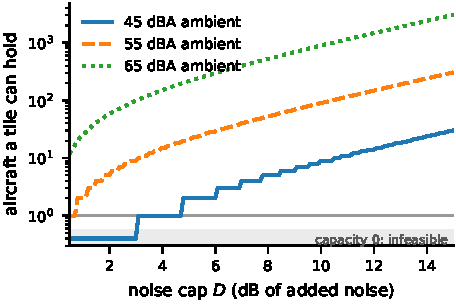
\includegraphics{figs/capacity.pdf}
\caption{Simultaneous overflights a community can absorb under a cap $D$ on
\emph{added} noise, by ambient level, from \eqref{eq:capclosed}. The cap is
baseline-independent; the capacity it implies is not. At $D=\SI{3}{\dB}$ a
\SI{45}{\dBA} community can host no aircraft at all, while a \SI{65}{\dBA} one can
host 99.}
\label{fig:capacity}
\end{figure}

\paragraph{Disparity cap $U$} At any timestep, the spread of added noise across tiles
may not exceed $U$. The direct statement is pairwise,
\begin{equation}
\bigl|\dbinc_{m_1}(c_{m_1,t}) - \dbinc_{m_2}(c_{m_2,t})\bigr| \le U
\quad \forall\, m_1,m_2,t ,
\label{eq:upair}
\end{equation}
which requires a conditional table over every \emph{ordered pair} of tiles and every
count value --- $O(M^2 \capm)$ implications per timestep. We instead use the identity
\begin{equation}
\eqref{eq:upair} \iff \max_m \dbinc_m(c_{m,t}) - \min_m \dbinc_m(c_{m,t}) \le U
\end{equation}
and introduce two auxiliary integers per timestep:
\begin{equation}
\overline{d}_t \ge \tilde\dbinc_m(c_{m,t}),\quad
\underline{d}_t \le \tilde\dbinc_m(c_{m,t}) \ \ \forall m, \quad
\overline{d}_t - \underline{d}_t \le \tilde U .
\label{eq:ucap}
\end{equation}
This is sound and complete. Soundness: $\overline{d}_t$ is forced at or above the true
maximum and $\underline{d}_t$ at or below the true minimum, so bounding their difference
bounds the true spread. Completeness: any assignment whose true spread fits within $U$
is satisfiable by setting the auxiliaries to the actual extremes. The cost falls to
$2M+1$ constraints per timestep, and the conditionals it refers to are the ones the
objective terms need anyway, so the disparity cap adds no new nonlinear terms at all.

\begin{table}[t]
\centering
\caption{The two disparity encodings, built on an otherwise identical phase-2 model and timed. Both state the same constraint and agree on the objective at every size. The pairwise form needs two orders of magnitude more assertions and takes correspondingly longer to \emph{build}, but it \emph{solves} $6$--$9\times$ faster --- so the max/min encoding's advantage is in construction, and it decays from $3.2\times$ on total time at $N{=}6$ to parity at $N{=}16$. Single runs on an idle machine; the solve times at $N{=}6$ are under a second and should be read as indicative.}
\label{tab:pairwise}
\begin{tabular}{r rr rr rr}
\toprule
\multirow{2}{*}{$N$} & \multicolumn{2}{c}{max/min} & \multicolumn{2}{c}{pairwise} & \multicolumn{2}{c}{ratio} \\
\cmidrule(lr){2-3}\cmidrule(lr){4-5}\cmidrule(lr){6-7}
 & constr. & solve (s) & constr. & solve (s) & solve & total \\
\midrule
6 & 306 & 0.64 & 25,200 & 0.12 & $0.19\times$ & $3.22\times$ \\
8 & 306 & 1.28 & 32,400 & 0.20 & $0.16\times$ & $2.31\times$ \\
14 & 306 & 4.47 & 48,240 & 0.47 & $0.11\times$ & $1.17\times$ \\
16 & 306 & 6.11 & 53,136 & 0.72 & $0.12\times$ & $1.00\times$ \\
\bottomrule
\end{tabular}
\end{table}


The constraint counts differ by two orders of magnitude, and we initially reported that
ratio as though it were a speedup. Building both encodings on an otherwise identical
model and timing them says otherwise (Table~\ref{tab:pairwise}). The two agree on the
objective at every size, confirming they state the same constraint. But the pairwise
encoding \emph{solves} $6$--$9\times$ \textbf{faster}: giving Z3 the disparity relation
explicitly, rather than through two auxiliary variables it must reason about, evidently
helps its search. What max/min buys is \emph{construction} time --- 306 assertions
against tens of thousands --- and that advantage decays with fleet size, from
$3.2\times$ on total time at $N=6$ to exactly $1.0\times$ at $N=16$. Extrapolating the
trend, the pairwise form would win outright at the fleet sizes we most care about.

We report this because the honest conclusion contradicts the one we started with. The
max/min encoding is worth keeping at workshop scale, where a solve is dominated by
construction and the tool must feel responsive; it is not what makes these problems
tractable, and the constraint-count ratio was never evidence that it was. Constraint
counts are a proxy for encoding cost, not for search cost, and the two came apart here in
the direction opposite to the intuition.

\subsection{Horizon selection and the two-phase solve}
\label{sec:softT}

$T$ is not given. Too small and the instance is spuriously infeasible; too large and
every extra timestep replicates the entire noise encoding for all $M$ tiles. We
therefore solve in two phases.

\emph{Phase 1} finds the smallest feasible horizon. A lower bound $T_{\min}$ comes from
a breadth-first search per aircraft restricted to \emph{$D$-admissible} tiles, those
with $\capm_m \ge \mu_i$; this is a sound necessary condition because it ignores all
interaction between aircraft and so can only under-constrain. The encoding is then built
once at $T_{\min}$ and extended by a single timestep per iteration, with the destination
pins $L_{i,T-1} = e_i$ asserted as \emph{assumption literals}. This lets the unsat core
distinguish the two ways an instance can fail: if no destination assumption appears in
the core, the conflict is structural and no horizon will ever help, so the search stops
immediately instead of grinding to its cap.

\emph{Phase 2} fixes the horizon and optimises. Under a \emph{soft} horizon the phase-2
horizon is set above $T_{\min}$, giving aircraft room to stagger their arrivals rather
than all being airborne simultaneously; arrival is then made sticky,
\begin{equation}
\mathrm{ha}_{i,t} \Rightarrow L_{i,t+1} = e_i ,
\label{eq:sticky}
\end{equation}
so an aircraft that lands early stays landed instead of drifting. Constraint
\eqref{eq:sticky} is why self-loops in $A$ are mandatory: without $A_{e_ie_i}=1$ a
landed aircraft would have no legal move and the instance would be trivially
unsatisfiable.

\subsection{Mapping the five principles}
\label{sec:mapping}

Table~\ref{tab:mapping} summarises the translation; the five subsections that follow give
each principle separately, since what each one needs from the model differs more than a
shared notation suggests. Throughout, $P \subseteq \stations$ is a protected set, $w_m$ a
per-tile transit weight, and $\pi_m$ a per-tile price. Every objective is minimised.

%% Hand-written (unlike the rest of tables/, which analyze.py generates).
%% This is the paper's central claim about the encoding, not a measurement.
\begin{table*}[t]
\centering
\caption{The five principles as constraints. ``Form'' is whether the principle's own
statement is a satisfaction condition or an optimisation; ``Encoded as'' is what our
solver receives. The one row where these disagree is Equal, and
Section~\ref{sec:mismatch} measures what that disagreement costs. $\ell$ is the
user-selected decibel limit, $P$ the protected set, $\pi_m$ the benefit-derived price
of \eqref{eq:price}, and $\infty$ a cap set wide enough to be unreachable.}
\label{tab:mapping}
\begin{tabular}{llllc}
\toprule
Principle & Statement in this domain & Form & Encoded as & Objective? \\
\midrule
Equal &
  added noise as equal as possible across communities &
  optimisation &
  hard cap $U \le \ell$ (and $D \le \ell$) &
  no \\
Sufficientarian &
  no community's noise exceeds a stated threshold &
  satisfaction &
  hard cap $D \le \ell$, $U \le \infty$ &
  no \\
Prioritarian &
  the already most-burdened receive the least additional noise &
  optimisation &
  $\min J_{\mathrm{prior}} = \sum_{t}\sum_{p \in P} \tilde\dbinc_p(c_{p,t})$ &
  yes \\
Utilitarian &
  the summed added noise over all communities is lowest &
  optimisation &
  $\min J_{\mathrm{util}} = \sum_{t}\sum_{m} w_m \tilde\dbinc_m(c_{m,t})$ &
  yes \\
Proportional &
  those who benefit most from the network carry more of its noise &
  optimisation &
  $\min J_{\mathrm{prop}} = \sum_{t}\sum_{m} \pi_m\,\tilde\dbinc_m(c_{m,t})$ &
  yes \\
\bottomrule
\end{tabular}
\end{table*}


\subsubsection{Equal}
\label{sec:enc-equal}
Equal constrains differences between communities, so it is the one principle that needs a
quantity no single community possesses. We bound the spread of added noise at every
timestep,
\begin{equation}
\max_m \dbinc_m(c_{m,t}) - \min_m \dbinc_m(c_{m,t}) \;\le\; \ell
\quad \forall t ,
\label{eq:enc-equal}
\end{equation}
which is the disparity cap $U = \ell$ of \eqref{eq:ucap}, and we contribute no objective
term. This takes the satisfaction reading of Equal identified in
Section~\ref{sec:p-equal}. It is the cheaper reading --- \eqref{eq:ucap} costs $2M+1$
linear constraints per timestep, against an optimisation over $\max_m - \min_m$ which
would add a further objective tier --- and it is the reading the deployed tool takes.
Section~\ref{sec:mismatch} measures what it costs, and the cost is not small.

\subsubsection{Sufficientarian}
\label{sec:enc-suff}
Sufficientarian constrains each community's own increase against a threshold, with no
reference to any other community:
\begin{equation}
\dbinc_m(c_{m,t}) \;\le\; \ell \quad \forall m,t ,
\label{eq:enc-suff}
\end{equation}
which is the absolute cap $D = \ell$, enforced through the count bound \eqref{eq:dcap}.
Again no objective term, and here that is faithful rather than a compromise:
Sufficientarianism is natively a satisfaction condition and is genuinely silent among
distributions that clear the threshold. Of the five this is the only principle whose form
survives the encoding untouched.

\subsubsection{Prioritarian}
\label{sec:enc-prior}
Prioritarian needs an input the noise model does not contain --- an identification of the
already worst-off --- which enters as an explicit protected set $P$. It then minimises
the noise those communities receive:
\begin{equation}
J_{\mathrm{prior}} \;=\; \sum_{t}\sum_{p \in P} \tilde\dbinc_p(c_{p,t}) .
\label{eq:jprior}
\end{equation}
Two properties follow from the shape of \eqref{eq:jprior} and both are visible in
Section~\ref{sec:degeneracy}. It is bounded below by zero and \emph{attains} zero whenever
a routing exists that never overflies $P$, after which it expresses no further
preference --- so it behaves as a hard exclusion wearing an objective's clothing. And
because it is silent about every community outside $P$, it says nothing about where the
displaced traffic goes.

We choose $P$ as the three loudest non-vertiport communities, following the source
document's ``regions that presently and historically bear the greatest noise burden from
existing transportation infrastructure''. Vertiports are excluded because every flight
must land at one, which would make the objective unsatisfiable rather than binding.

\subsubsection{Utilitarian}
\label{sec:enc-util}
Utilitarian aggregates, so it sums the added noise over every community and timestep:
\begin{equation}
J_{\mathrm{util}} \;=\; \sum_{t}\sum_{m} w_m\,\tilde\dbinc_m(c_{m,t}) ,
\label{eq:jutil}
\end{equation}
with $w_m \equiv 1$ unless the deployment weights communities by population. This is the
most direct of the five translations --- the principle names a sum, and the encoding is
that sum --- and it inherits the principle's indifference to distribution exactly:
\eqref{eq:jutil} cannot distinguish one community bearing $20$ units from twenty bearing
one. Combined with the concavity and baseline-dependence of \eqref{eq:db}, that
indifference has consequences we quantify in Section~\ref{sec:concavity}.

\subsubsection{Proportional}
\label{sec:enc-prop}
Proportional is relational: it ties burden to benefit, and benefit is not in the noise
model at all. Section~\ref{sec:proportional-encoding} constructs a per-tile price $\pi_m$
from participants' own ranking of what confers benefit; given it, the objective is
\begin{equation}
J_{\mathrm{prop}} \;=\; \sum_{t}\sum_{m} \pi_m\,\beta_{m,t} ,
\label{eq:jprop}
\end{equation}
where $\beta_{m,t}$ is a burden measure defined below. Because $\pi_m$ is
\emph{constructed} rather than measured, this is the one principle whose encoding embeds
a second set of contestable judgements on top of the principle itself --- which is why we
make the construction an explicit input rather than a constant.

\subsubsection{Arrival time, which is not a principle}
\label{sec:enc-time}
Independently of the five, aircraft should not loiter. We count pre-arrival
aircraft-timesteps,
\begin{equation}
J_{\mathrm{time}} \;=\; \sum_{i}\sum_{t} [\,\neg\,\mathrm{ha}_{i,t}\,] ,
\label{eq:jtime}
\end{equation}
a proxy for total travel time. This is an efficiency term, not a fairness one, and
Section~\ref{sec:normalisation} explains why it is kept strictly subordinate to whichever
principle is selected.

\subsection{Constructing ``benefit'' for the Proportional principle}
\label{sec:proportional-encoding}

Proportional requires a quantity the noise model does not contain. We construct it
explicitly, as a price $\pi_m$ that the objective pays for each unit of burden borne by
tile $m$; minimising $J_{\mathrm{prop}}$ therefore pushes traffic \emph{toward} cheap
tiles, so a low price means ``benefits from the system, should carry noise'' and a high
price means ``protected''.

Participants rank $F$ plain-language factors --- in our instantiation income, current
ambient level, distance to the nearest vertiport, and population. Each factor $f$ scores
every tile on a common scale $\sigma_f(m) \in [0,\Sigma]$ where $0$ means ``overfly
freely'' and $\Sigma$ means ``protect''. A rank order induces weights $\rho_f$ summing
to one, and
\begin{equation}
\pi_m \;=\; \gamma^{\;\sum_{f} \rho_f\,\sigma_f(m)}
       \;=\; \prod_{f} \gamma^{\,\rho_f \sigma_f(m)} ,
\label{eq:price}
\end{equation}
with base $\gamma$. The product form is deliberate: each factor contributes its own
multiplicative factor, so a price reads back as the separate contribution of each ranked
choice rather than one opaque number. Since $\sum_f \rho_f = 1$ and
$\sigma_f \in [0,\Sigma]$, the price stays in $[1,\gamma^\Sigma]$ however participants
rank. The distance factor's \emph{sign} is the principle: proximity to a vertiport scores
as cheap, because the tiles nearest a vertiport enjoy the access and so under
benefit-carries-burden are the ones that should pay. A prototype that scored proximity as
deserving protection was implementing the opposite principle.

The burden measure $\beta_{m,t}$ admits two non-interchangeable choices. \emph{Occupancy},
$\beta_{m,t} = c_{m,t}$, charges each aircraft-timestep that tile's price linearly; being
separable across aircraft it is far cheaper to optimise. \emph{Decibel},
$\beta_{m,t} = \tilde\dbinc_m(c_{m,t})$, charges the noise the community actually
experiences --- the more defensible reading, and our default. The decibel form inherits
both awkward properties of \eqref{eq:db}: concavity makes the objective \emph{prefer} to
concentrate traffic, and baseline-dependence applies the $\approx\!70\times$ gradient
toward loud tiles on top of whatever ambient preference participants expressed,
double-counting a factor they were asked to rank. We flag the trade rather than resolving
it: which reading is correct is a normative question our measurements can inform but not
settle.

\subsection{Normalisation and the priority between constraints}
\label{sec:normalisation}

The terms in \eqref{eq:jutil}--\eqref{eq:jtime} have incommensurable units --- summed
centi-decibels, priced occupancy, aircraft-timesteps. Each is therefore divided by an
upper bound on its own value, so that a stated weight of $1.0$ means the same thing
across terms:
\begin{equation}
\hat{J}_k = J_k / J_k^{\max}, \qquad
J_{\mathrm{tier1}} = \sum_k \omega_k \hat{J}_k .
\end{equation}
These bounds must be \emph{tight}, not merely valid: a loose divisor produces no error,
it silently shrinks a term's reachable range, so a weight the user set to $1.0$ behaves
like a much smaller number and the routing stops responding to it. The obvious bound for
$J_{\mathrm{prop}}$ --- every tile simultaneously carrying the whole fleet --- needs
$M\sum_i \mu_i$ aircraft when only $\sum_i \mu_i$ exist, and overstates the attainable
maximum by $16.4\times$ here. We instead compute the exact single-timestep maximum by
bounded-knapsack dynamic programming, rather than greedy marginal allocation, precisely
because rounding destroyed concavity (Section~\ref{sec:noise}) and greedy would
under-estimate --- the harmful direction.

\paragraph{Priority.} Folding $J_{\mathrm{time}}$ into the same weighted sum as the
principle terms makes the outcome depend on how tight each normalising bound happens to
be, which is a property of the bounds rather than of the ethics. An earlier version of
this system did exactly that: instrumenting it showed the time term occupying $68.8\%$ of
its normalised range against the utilitarian term's $2.2\%$, so with every stated weight
at $1.0$ the solver was in effect minimising arrival time alone, at roughly $31\!:\!1$
against the selected principle.\footnote{Measured on the superseded weighted scheme and
reported as the motivation for replacing it; no result in Section~\ref{sec:results}
depends on it.}

We therefore make the objective \textbf{lexicographic}: the principle tier is minimised
first, and arrival time is minimised only among routings that already achieve the
principle's optimum. Travel time then provably cannot cost a single unit of fairness. It
still does real work, because the principle tiers are massively degenerate --- often
thousands of routings share the optimal principle value --- and arrival time selects
among them.

Two consequences follow. When only one principle term is live, that term's weight cannot
move the argument minimum: scaling a lone principle weight is mathematically inert, and an
interface offering the dial is offering a placebo (two live terms still trade at their
stated ratio). And the principle tier is a harder problem than the blended one, so
timeouts become more common --- though an unproven answer under this scheme can still be
better than a proven answer under the other.

\paragraph{When the clock runs out} A fairness tool that degrades silently is worse than
one that fails loudly, because the degraded answer still looks like an answer. A phase-2
timeout usually leaves an incumbent that satisfies every hard constraint and has the
objective applied, and is merely unproven; we salvage it, \emph{re-verify it against the
full constraint set} rather than trusting it, and mark it \texttt{partial}. Only when no
incumbent exists does the system fall back to phase 1's unweighted route, and that
outcome is flagged, because a routing that ignores the selected principle must never be
presented beside one that does not.

\section{Results}
\label{sec:results}

\subsection{Setup}
\label{sec:setup}

The instance is a $5\times5$ grid of $M=25$ communities drawn from Austin, TX, each
carrying an ambient level of \SI{45}{\dBA} (8 tiles), \SI{55}{\dBA} (12) or
\SI{65}{\dBA} (5). Three tiles host vertiports --- an airport, a downtown core and an
exurban commuter town --- and traffic runs in both directions on all three
origin--destination pairs. The per-aircraft source level is \SI{45}{\dBA} and one
timestep is \SI{180}{\second}. Fleet size is set by a demand factor, giving the ladder
$N \in \{6,8,14,16,22,24,30,32\}$.

We compare six conditions at every size: the five principles, and a \emph{baseline} ---
the same fleet with the caps opened and every objective cleared, which is the
shortest-time routing the solver returns when no principle has been selected. It is the
zero against which everything here is measured.

\paragraph{The operating point, and why it is not the default} The cap, the protected set
and the objective encoding are set so that each principle constrains the routing on the
fleet range studied. The cap is $D=\SI{6}{\dB}$ of added noise, applied to all five
principles so they face one hard constraint and differ only in their objective; the
Prioritarian protected set is the three busiest non-vertiport communities that are also
low-income. Both choices are forced. At the settings the system ships with --- $D=10$,
and a protected set chosen as the loudest tiles --- the caps sit at a third of the
capacity they allow, and the protected set carries \emph{zero} aircraft-timesteps at every
fleet size, so its objective is satisfied without the routing changing at all. In that
regime Equal and Sufficientarian return the baseline's routing exactly at $N=8$ and
differ from it by less than the solver's own indifference above.
Choosing an operating point at which a principle does something is a precondition for
measuring what it does, not a result.

Utilitarian and Proportional run the count-weighted form of their objectives
(Section~\ref{sec:encoding}), which the solver already exposes. The decibel form does not
prove optimality above $N=8$ on any budget we gave it; the count form proves every cell
we ran, faster by $51\times$ at $N=8$ for Utilitarian and $1110\times$ for Proportional.
That difference belongs to the encoding, not to the principle, and
Section~\ref{sec:tractability} returns to it.

\paragraph{Every cell is four solves} A single solve is one draw from a set of
equally-optimal routings, and which member comes back is decided by the order the
aircraft happen to be listed in. Every cell here is therefore solved four times under
four permutations of that list. A permutation leaves the fleet, the origin--destination
pairs and the feasible set identical, so the spread across the four is the solver's
indifference and nothing else. The permutation at index $k$ is the same for every
condition, so comparisons at fixed $k$ are paired.

That spread is drawn as a band on every curve, and it fixes what counts as a finding: a
difference between two conditions is reported only when their means differ by more than
the larger of their two bands \emph{and} the bands do not overlap. Differences inside the
band are stated as within the tie-break and nothing is built on them.

\paragraph{Budget} Every solve ran unlimited. A cell that had not proved after
\SI{3600}{\second} was stopped and its incumbent salvaged --- a routing satisfying every
hard constraint, verified before being served, but not proven optimal. The horizon is
uniform, so the proof frontier is a property of the problem. Proven cells are filled
markers and carry bands; harvested cells are hollow, carry no band, and are never joined
to a curve.

\subsection{Routing and congestion as the fleet grows}
\label{sec:degeneracy}

Fig.~\ref{fig:routes-grid} shows the map at four fleet sizes, one column per condition.
Through $N=24$ every condition is proven optimal in all four permutations.

The first thing the bands settle is that congestion does \emph{not} separate the
principles. Peak aircraft over one community rises from 2 to roughly 13 for every
condition, and the bands on it are 3 to 6 aircraft wide --- wider than any gap between
conditions. The single exception is Proportional, which is attributable at $N=8$ and,
more tellingly, carries a band of exactly zero at every fleet size: it places 3, 5, 8,
10, 12 and 14 aircraft on its busiest tile, the same number in all four permutations.
Everywhere else, an ordering of the traffic that no one chose moves the peak occupancy
more than the choice of principle does.

\subsection{Travel time: two families, two currencies}
\label{sec:traveltime}

Through $N=16$ no condition flies further than the shortest-path floor. Above it the
principles begin to pay, and they pay in different coin.

The three cap-based principles pay in distance. Averaged over the four permutations, at
$N=22$ and $N=24$ Equal flies 2.75 fleet-hops above the baseline, Sufficientarian 3.00
and 2.75, and Prioritarian 2.50 --- individual runs are 2 or 3 hops, and the difference
from the baseline's zero is attributable at every one of those six cells. The two
objective-based principles fly \emph{no} extra distance at any size, in any permutation,
and instead depart later: 25 and 27 aircraft-timesteps of departure delay at $N=22$ and
$N=24$ against the baseline's 22 and 24, with zero band on both sides. They de-conflict
the fleet in time rather than routing it apart in space.

This is why travel time has to be reported as two quantities. A study that counted only
hops would record the objective principles as free, and one that counted only arrival
time would miss that the caps are buying their result by rerouting. Both panels of
Fig.~\ref{fig:metric-vs-N} are needed, and Table~\ref{tab:response} reports both.

\subsection{Noise: a binding cap makes the outcome determinate}
\label{sec:concavity}

The central result of this section is not that the principles are quieter than the
baseline. It is that they are \emph{reliably} quieter, and the baseline is not reliably
anything.

From $N=14$ upward, every one of the five principles returns a peak added level of
exactly \SI{4.77}{\dB}, in all four permutations, at every fleet size. The band is zero.
The baseline over the same range returns 5.64, 5.88, 6.70 and \SI{7.70}{\dB} with bands
of 2.22, 2.22, 1.76 and \SI{3.98}{\dB} --- its peak is whatever the tie-break happens to
produce. At $N=22$ the gap clears the band for all five principles.

The mechanism is the interaction of the cap with an integer capacity. Inverting
$\dbinc_m$ in \eqref{eq:cap} gives the capacity a cap grants a tile in closed form,
\begin{equation}
\capm_m \;=\; \Bigl\lfloor \bigl(10^{D/10} - 1\bigr)\,
              10^{(b_m - \alpha)/10} \Bigr\rfloor ,
\label{eq:capclosed}
\end{equation}
which is exactly two aircraft for a \SI{45}{\dBA} community at $D=\SI{6}{\dB}$ --- and
the routing saturates it. Two aircraft over a quiet tile add \SI{4.77}{\dB}, which is the
number every principle returns. A cap that binds does not merely lower the worst outcome,
it \emph{determines} it, because the binding constraint and not the search decides where
the peak sits. That is a property a community could rely on, and the un-capped routing
does not have it.

\label{sec:mismatch}
It also explains why Equal and Sufficientarian are indistinguishable here. Equal bounds
the \emph{spread} of added noise across communities and Sufficientarian bounds its
\emph{level}, and those are different rules about different things --- but encoded as the
caps $U \le \ell$ and $D \le \ell$ they are not.

\begin{proposition}[Collapse]
\label{prop:collapse}
Let $F_D(\ell)$ denote the set of routings satisfying
$\max_{m,t}\dbinc_m(c_{m,t}) \le \ell$ and $F_U(\ell)$ those satisfying
$\max_m \dbinc_m(c_{m,t}) - \min_m \dbinc_m(c_{m,t}) \le \ell$ for every $t$. Then
$F_D(\ell) \subseteq F_U(\ell)$.
\end{proposition}
\begin{proof}
$\dbinc_m(n) \ge 0$ for all $m,n$, since $\dbinc_m(0)=0$ and $\dbinc_m$ is increasing.
Hence $\min_m \dbinc_m(c_{m,t}) \ge 0$ and
$\max_m \dbinc_m - \min_m \dbinc_m \le \max_m \dbinc_m \le \ell$.
\end{proof}

The inclusion is not specific to noise: a bound on the spread of any non-negative
quantity is implied by a bound on its level, so wherever a system offers both, the
comparative cap is the weaker of the two. Below $N=25$ the two principles are sent
$(D,U)=(\ell,\ell)$ and $(\ell,\infty)$, which this reduces to the same feasible set, and
no measurement here separates them.

Summed added noise separates differently, and here Proportional is the outlier in the
study. Its total added noise is attributable against the baseline at five of the six
proven sizes --- \SI{10.9}{\dB} against \SI{17.6}{\dB} at $N=6$, \SI{29.0}{\dB} against
\SI{47.9}{\dB} at $N=24$ --- and its band is zero at every size. Pricing the burden per
community, even over plain counts, produces both the largest reduction in total exposure
and the only routing in the study that is fully determined at every fleet size.
Prioritarian is attributable at $N=14$ and $16$ (\SI{28.0}{\dB} against \SI{37.7}{\dB}),
buying its reduction by keeping traffic off three named communities.

\subsection{Solver performance}
\label{sec:tractability}

The tractability ordering reported in earlier work inverts once the encoding is stated.
In count form, Utilitarian is the \emph{cheapest} of the six conditions to solve at every
size through $N=16$ --- \SI{1.6}{\second} at $N=6$ and \SI{8.5}{\second} at $N=16$,
against \SI{5.9}{\second} and \SI{55.3}{\second} for the baseline, which carries no
fairness term at all. Its objective prunes the search rather than extending it. The three
cap-based conditions and the baseline run together, 35 to \SI{200}{\second} through
$N=24$. Proportional is the most expensive, reaching \SI{438.6}{\second} at $N=24$,
because its price vector gives every community a distinct weight and so removes the
symmetry the other objectives leave intact.

Above $N=24$ the ladder thins, and the two caps part company. Above $N=25$ the system
stops sending an absolute cap to Equal and sends a bound on the \emph{spread} between
communities instead; under that bound no Equal cell at $N=30$ or $32$ produced a routing
its own phase-2 search could verify, within the harvest horizon, in any permutation. The
absolute cap does not have this problem: Sufficientarian returns verified routings at both
sizes. A comparative cap and an absolute one are interchangeable when neither binds
(Proposition~\ref{prop:collapse}); at the top of this ladder only one of them is solvable.

\subsection{Summary}

\emph{Equal} and \emph{Sufficientarian} do nothing below $N=14$, then pin the worst-hit
community at \SI{4.77}{\dB} and pay 3 fleet-hops for it from $N=22$; they are
indistinguishable from each other throughout, which Proposition~\ref{prop:collapse}
predicts. \emph{Prioritarian} does the same on peak while also cutting total exposure at
$N=14$ and $16$, for 2 hops. \emph{Utilitarian} is free in distance, pays 3
aircraft-timesteps of departure delay, and is the cheapest condition in the study to
solve. \emph{Proportional} is the only principle whose routing is fully determined at
every fleet size, and it removes the most total exposure, at the highest computational
price.

Across all five, what the choice of principle buys on this instance is not a quieter map
so much as a \emph{predictable} one: five constrained routings that return the same peak
every time, against an unconstrained routing that varies by up to \SI{3.98}{\dB}
depending on nothing anyone selected.

\begin{figure*}[t]
\centering
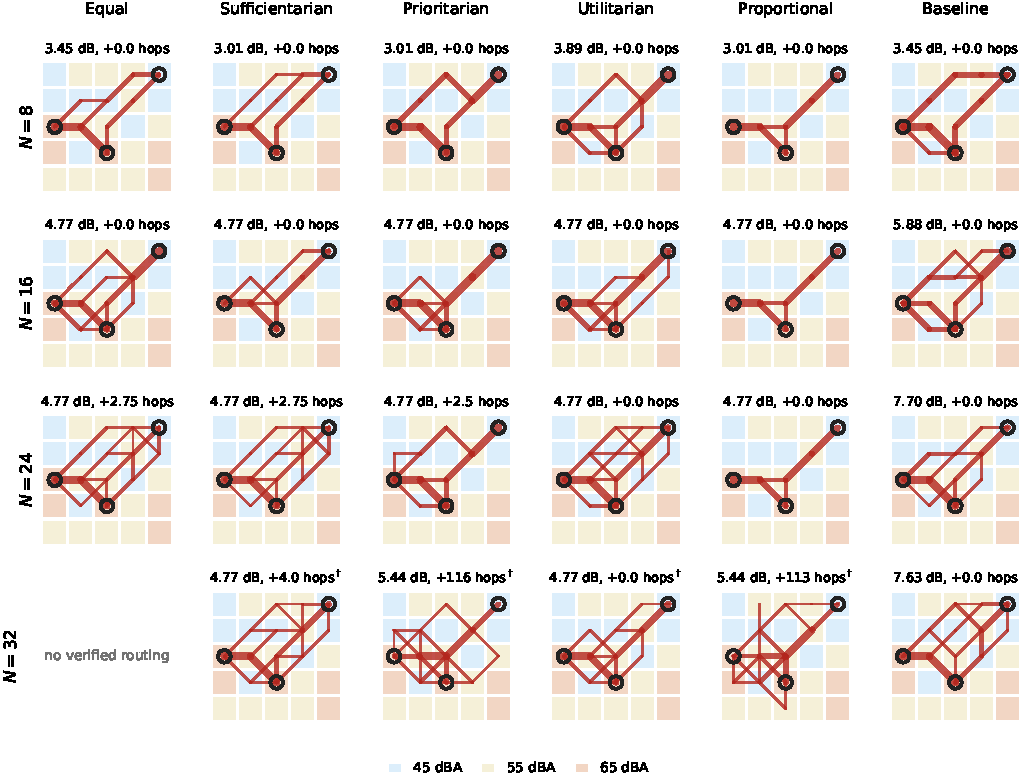
\includegraphics{figs/routes_grid.pdf}
\caption{The instance at four fleet sizes, one column per condition. Tiles are shaded by
ambient level, vertiports ringed, and each panel overlays every aircraft's path with line
width proportional to the aircraft on that leg, for one representative permutation.
Because the widths sum over the horizon, two panels can look alike while the routings
differ in \emph{when} each leg is flown. A dagger marks a cell that was harvested at the
budget horizon rather than proven.}
\label{fig:routes-grid}
\end{figure*}

\begin{figure*}[t]
\centering
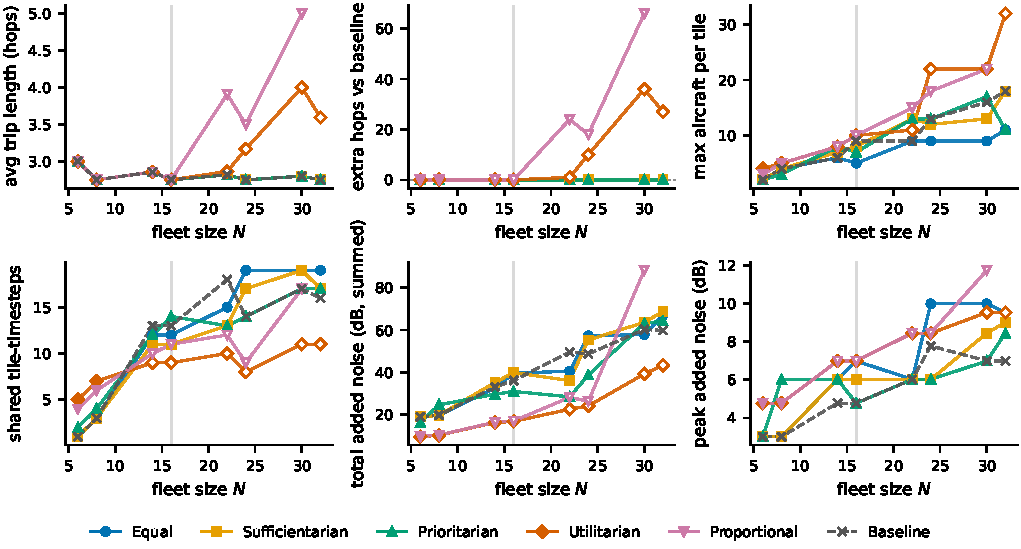
\includegraphics{figs/metric_vs_N.pdf}
\caption{Six metrics against fleet size. Each line runs through the mean of four
permutations of the aircraft list and the shaded band is their full range --- the
solver's indifference at that cell. Two conditions whose bands overlap are not separated
by anything the principle did. Lines join proven cells only; harvested cells appear as
isolated hollow markers, since a stopped search sits at an unknown distance from the
optimum and joining it to the curve would draw a trend out of how far the solver got.}
\label{fig:metric-vs-N}
\end{figure*}

\begin{table}[t]
\centering
\caption{How each principle responds to fleet size. \emph{From} is the smallest fleet at which the principle's routing differs from the no-fairness baseline by more than the permutation band at that cell; the arrow is whether that difference grows or shrinks above it. A dash means the principle never separates from the baseline on that metric, which is a property of the principle on this instance rather than a missing measurement.}
\label{tab:response}
\begin{tabular}{lllll}
\toprule
Principle & Congestion & Travel Time & Departure Delay & Added Noise \\
\midrule
Equal & -- & $-$ from $N{=}22$ & -- & $-$ from $N{=}22$ \\
Sufficientarian & -- & $-$ from $N{=}22$ & -- & $-$ from $N{=}22$ \\
Prioritarian & -- & $-$ from $N{=}22$ & -- & $-$ from $N{=}22$ \\
Utilitarian & -- & -- & $\uparrow$ from $N{=}22$ & $\uparrow$ from $N{=}22$ \\
Proportional & $-$ from $N{=}8$ & -- & $-$ from $N{=}22$ & $-$ from $N{=}22$ \\
\bottomrule
\end{tabular}
\end{table}


\begin{table}[t]
\centering
\caption{Routing under each principle as the fleet grows, on setup \texttt{D6\_protA} at an unlimited solver budget. \emph{+vs base} is total fleet hops above the no-fairness baseline at the same $N$; \emph{max/tile} the largest number of aircraft over one community at one timestep; \emph{shared} the tile-timesteps carrying two or more. Total added noise is the arithmetic dB sum the Utilitarian term minimises. A dagger marks a verified feasible routing whose optimality is unproven; every such number bounds the optimum rather than stating it.}
\label{tab:fleet-main}
\begin{tabular}{r l rr rr rr}
\toprule
$N$ & Condition & avg hops & +vs base & max/tile & shared & total dB & peak dB \\
\midrule
8 & Equal & 2.75 & 0 & 4 & 4 & 20.0 & 3.45 \\
8 & Sufficientarian & 2.75 & 0 & 4 & 3 & 19.6 & 3.01 \\
8 & Prioritarian & 2.75 & 0 & 4 & 5 & 17.0 & 3.01 \\
8 & Utilitarian & 2.75 & 0 & 3 & 5 & 20.4 & 3.89 \\
8 & Proportional & 2.75 & 0 & 5 & 5 & 11.6 & 3.01 \\
8 & Baseline & 2.75 & 0 & 4 & 4 & 19.4 & 3.45 \\
\midrule
16 & Equal & 2.75 & 0 & 8 & 14 & 35.0 & 4.77 \\
16 & Sufficientarian & 2.75 & 0 & 8 & 12 & 34.8 & 4.77 \\
16 & Prioritarian & 2.75 & 0 & 8 & 13 & 28.0 & 4.77 \\
16 & Utilitarian & 2.75 & 0 & 7 & 14 & 39.3 & 4.77 \\
16 & Proportional & 2.75 & 0 & 10 & 13 & 19.7 & 4.77 \\
16 & Baseline & 2.75 & 0 & 7 & 14 & 37.7 & 5.88 \\
\midrule
24 & Equal & 2.86 & 3 & 13 & 16 & 56.0 & 4.77 \\
24 & Sufficientarian & 2.86 & 3 & 13 & 16 & 56.0 & 4.77 \\
24 & Prioritarian & 2.85 & 2 & 12 & 17 & 40.3 & 4.77 \\
24 & Utilitarian & 2.75 & 0 & 11 & 18 & 53.9 & 4.77 \\
24 & Proportional & 2.75 & 0 & 14 & 16 & 29.0 & 4.77 \\
24 & Baseline & 2.75 & 0 & 12 & 15 & 47.9 & 7.70 \\
\midrule
32 & Sufficientarian & 2.88$^\dagger$ & 4$^\dagger$ & 17$^\dagger$ & 19$^\dagger$ & 73.0$^\dagger$ & 4.77$^\dagger$ \\
32 & Prioritarian & 6.38$^\dagger$ & 116$^\dagger$ & 25$^\dagger$ & 33$^\dagger$ & 114.9$^\dagger$ & 5.44$^\dagger$ \\
32 & Utilitarian & 2.75$^\dagger$ & 0$^\dagger$ & 16$^\dagger$ & 20$^\dagger$ & 61.5$^\dagger$ & 4.77$^\dagger$ \\
32 & Proportional & 6.28$^\dagger$ & 113$^\dagger$ & 25$^\dagger$ & 37$^\dagger$ & 118.3$^\dagger$ & 5.44$^\dagger$ \\
32 & Baseline & 2.75 & 0 & 16 & 17 & 55.2 & 7.63 \\
\bottomrule
\end{tabular}
\end{table}


% Generated and current, deliberately not \input: tables/reference.tex (the shipped
% default in three lines -- the one paragraph in IV-A covers it), tables/capacity.tex,
% figs/solve_time.pdf, figs/route_sharing.pdf, figs/noise_over_time.pdf, figs/floor.pdf.
% The same convention tables/caps.tex already follows. Re-add any if a reviewer asks.

\section{Discussion and Conclusion}
\label{sec:conclusion}

We encoded five principles of distributive justice as an explicit constraint system over
a multi-aircraft noise-routing problem, solved it with an optimising SMT solver, and
measured what each principle does. Five lessons generalise beyond our instance.

\paragraph{The encoding is part of the ethics} Equal admits both an optimisation reading
(``as equal as possible'') and a satisfaction reading (``no two communities differ by
more than $X$''); ordinary usage does not distinguish them, and taking the second --- the
cheaper, more composable choice --- left Equal returning answers interchangeable with
Sufficientarian's wherever the cap does not bind, so what looked like a choice between
principles was a choice between tie-breaks. Two conditions carry that result: no
objective term on either principle, and an optimum lying inside the tighter feasible set.
The first fails under the optimisation reading, which is why the collapse indicts the
reading rather than the principle. The second is empirical, but the underlying inclusion
is not specific to noise --- a bound on the \emph{spread} of any non-negative quantity is
implied by a bound on its \emph{level} --- so any system offering both a comparative and
an absolute fairness cap has one that can only ever be the weaker. A system offering a
menu of fairness principles owes a demonstration that the menu items are distinguishable,
and that is a claim about the instance, not a property of the code.

\paragraph{Ask whether a principle binds, not whether it is implemented} Whether a
principle does anything is a question about the operating point, not about the principle.
At the settings our system ships with, the caps sit at a third of the capacity they
allow and the protected set carries no traffic at all, and three of the five principles
then return the no-fairness routing or something indistinguishable from it. Move the cap
to where it binds and put the protected set where aircraft fly, and the same three
principles separate from that routing by margins a reader can act on.

Measuring which of those regimes one is in is cheap, and it is not the ablation we
started with. Re-solve the same configuration under permutations of the aircraft list:
the problem is unchanged, so the spread over those runs is the solver's indifference, and
a principle whose effect is smaller than that spread is not doing the work being
attributed to it. Running that test is how we found that our own deployed setting was the
wrong one to draw conclusions from.

\paragraph{An unproven answer is not a weak answer, it is a different kind of thing}
Four of our conclusions were wrong, all for the same reason: each compared a timed-out
incumbent against a proven optimum. At the deployed budget Equal and Sufficientarian
appeared to diverge at $N=30$ (arrival 149 against 147); a cap appeared to bind hard at
$N=32$ (158 against 88); Utilitarian appeared to fly more than the others over loud
communities; and the decibel-valued principles appeared to detour substantially from the
shortest path while the others did not. Given four hours, the first pair proves out
identical at 84 --- the earlier answers were $77\%$ from optimal --- the second at 88 with
no binding, the third vanishes, and the fourth reverses: wherever budgets are matched
($N \le 16$) \emph{all five} principles fly every aircraft on a shortest path, and the
apparent detour gap was an artefact of comparing four-hour rows for three principles
against \SI{600}{\second} rows for the other two. Every error pointed in the direction
that made the system look more interesting than it is, none was visible without
re-running, and none would have been caught by inspecting the routings.

We built a standing audit that grades each claim by the status of the rows beneath it,
and it caught the first two. It missed the last two, because it graded by \emph{status}
and the flaw was in \emph{budget}: a table can compare rows that are all `partial' and
still be confounded if some were given six hundred seconds and others four hours. The
audit now checks budget homogeneity within a comparison as well. We report this because
the failure is instructive --- an audit is only as good as the confound it was designed
against, and ours had to be taught a second one.

\paragraph{The metric carries a distributional judgement the principle does not}
Because sound adds in energy, expressing any fairness criterion in \emph{added}
decibels makes already-loud communities roughly $70\times$ cheaper to overfly than quiet
ones at our source level. Every principle we implemented inherits that gradient, and the
one optimising summed decibels most directly --- Utilitarian --- exploits it most, flying
least of all five over the quiet \SI{45}{\dBA} communities ($9.1\%$ of its flight time
against Equal's $34.1\%$) and displacing that traffic onto the mid-level ones. It does
\emph{not} fly more over the loudest tier: that share is pinned at $27.3\%$ for every
principle by where the vertiports sit. The gradient shows up as an exodus from the quiet,
not an influx to the loud. Nothing in the philosophical statement of utilitarianism says
``prefer communities that are already suffering''; the choice of measure says it. Since existing
noise burdens in the United States fall disproportionately on lower-income and minority
neighbourhoods~\cite{casey2017noise,simon2022sociodemographic}, a change-based metric
quietly ratifies the existing distribution. We do not claim an absolute-level metric is
correct; we claim the choice is normative and should be made explicitly.

\paragraph{Tractability is not neutral either} The principles expressible as hard caps
solved to proven optimality in under \SI{200}{\second} at fleet sizes where the two
decibel-valued optimisation principles could not prove optimality at all. If a
deployment picks its fairness rule partly on what it can compute in the time available
--- and a participatory tool with a room full of people waiting certainly does --- then
computational cost is silently doing normative work. Our system's response is to make
the three relevant facts machine-readable and visible: whether a principle was
optimised, whether its optimum was proven, and whether the answer on screen is the
principle's answer or a fallback that ignores it.

\subsection{Limitations and future work}

The acoustic model is deliberately coarse: a tile is treated as uniformly exposed over an
area several kilometres across, and aircraft are point sources with a single level, no
directivity, no altitude and no psychoacoustic weighting~\cite{nasaUAMnoise2020}. Absolute
decibel values should be read as ordinal. Our results concern how fairness rules order
routings under a given noise model, not how loud a real corridor would be.

Proposition~\ref{prop:collapse} holds for any instance, but the empirical findings are
measurements on two instances of one city. Our five principles are also five readings of
five traditions, fixed in advance by the definitions of
Section~\ref{sec:principles}; a maximin
Prioritarian, a threshold-then-Utilitarian Sufficientarian, or an Equal minimising
variance rather than range are all defensible, and comparing such variants is exactly
what this framework exists for. The most direct next step is to close the gap documented
here --- implement Equal as the minimisation its statement calls for, and measure what it
costs and whether it then separates from Sufficientarian. More broadly, the degeneracy we
observe suggests reporting a principle's whole optimal set rather than one arbitrary
member: the honest output of a fairness query may be a family of routings plus a
statement of what the principle does not determine.


\bibliographystyle{IEEEtran}
\bibliography{refs}

\end{document}
